\documentclass[12pt,oneside]{report}
\usepackage[a4paper,width=160mm,top=20mm,bottom=20mm]{geometry}

%\usepackage{fancyhdr}
%\pagestyle{fancy}

\usepackage[utf8]{inputenc}
\usepackage[english]{babel}
\usepackage{amsmath}
\usepackage{amsfonts}
\usepackage{natbib}
\usepackage{xcolor}
\definecolor{tab:blue}{RGB}{31, 119, 180}
\definecolor{tab:orange}{RGB}{255, 127, 14}
\definecolor{tab:green}{RGB}{44, 160, 44}
\definecolor{tab:red}{RGB}{214, 39, 40}
\usepackage{graphicx}
\graphicspath{ {images}}
\usepackage{nameref}
\usepackage[]{hyperref}
\usepackage{caption}
\usepackage{subcaption}

\newcommand{\mytitle}{On the representation of fluid-structure interaction by artificial neural networks in blast loadings} % Title here
\newcommand{\myauthor}{
Jørgen R. Høstmark\\~\\

Supervisors\\ 
David Morin\\
%Contracting authority:\\ SINTEF\\
%Open thesis\\
}

\title{\mytitle}
\author{\myauthor}
\date{\today}

\begin{document}

\begin{titlepage}
\begin{center}

\includegraphics[height=2cm]{0_Images/NTNU_hovedlogo_eng.png}\\[1cm]   
\end{center}
\begin{center}

 ~\\[1.5cm]

\textsc{\Large }\\[0.5cm] TKT4950 - Structural engineering \\ Master's thesis\\

 ~\\[.1cm]

\hrule ~\\[0.4cm]
{\huge \bfseries \mytitle}~\\[0.4cm]
\hrule ~\\[1.5cm]

\begin{minipage}{0.4\textwidth}
    \centering
	\large
	\myauthor
\end{minipage}

\vfill

{\large \today}

\end{center}
\end{titlepage}


\tableofcontents
\newpage
\chapter{Introduction} \label{chapter:Introduction}
Background, motivation and overview of thesis.
Blast loads can be unintentional (accidental explosion, Beirut explosion), or intentional (terrorism, IED, Oslo 2011). Want to design structures that are resilient to blast loads. Structures has the potential to protect people from blast loads, but structural collapse can cause harm. Example: Pakistan Mosque suicide bombing.
Fluid-structure interaction. Numerical simulation. Machine learning to represent fsi effects.
\newpage
\chapter{Theory}\label{CH2}

Blast load, what is it, how do we study it?
Experiments, simulations.
Artifical neural networks as universal function approximators, the mathematics and implementation.
\newpage
\chapter{Method} \label{chapter:Method}
Run simulations of plates with defects using cheap FSI by multiplying the lagrangian pressure with cosine of angle. Train a ANN and see if it can replicate this cheap FSI, (it should pretty much 100\%). Integrate the neural net with abaqus.

Simulate the plate using fully coupled FSI in Europlexus. Train an AI on this. Evaluate. Investigate if the material properties can be accounted for in the neural net.

\begin{figure}
    \centering
    \begin{subfigure}[b]{0.6\textwidth}
        \centering
        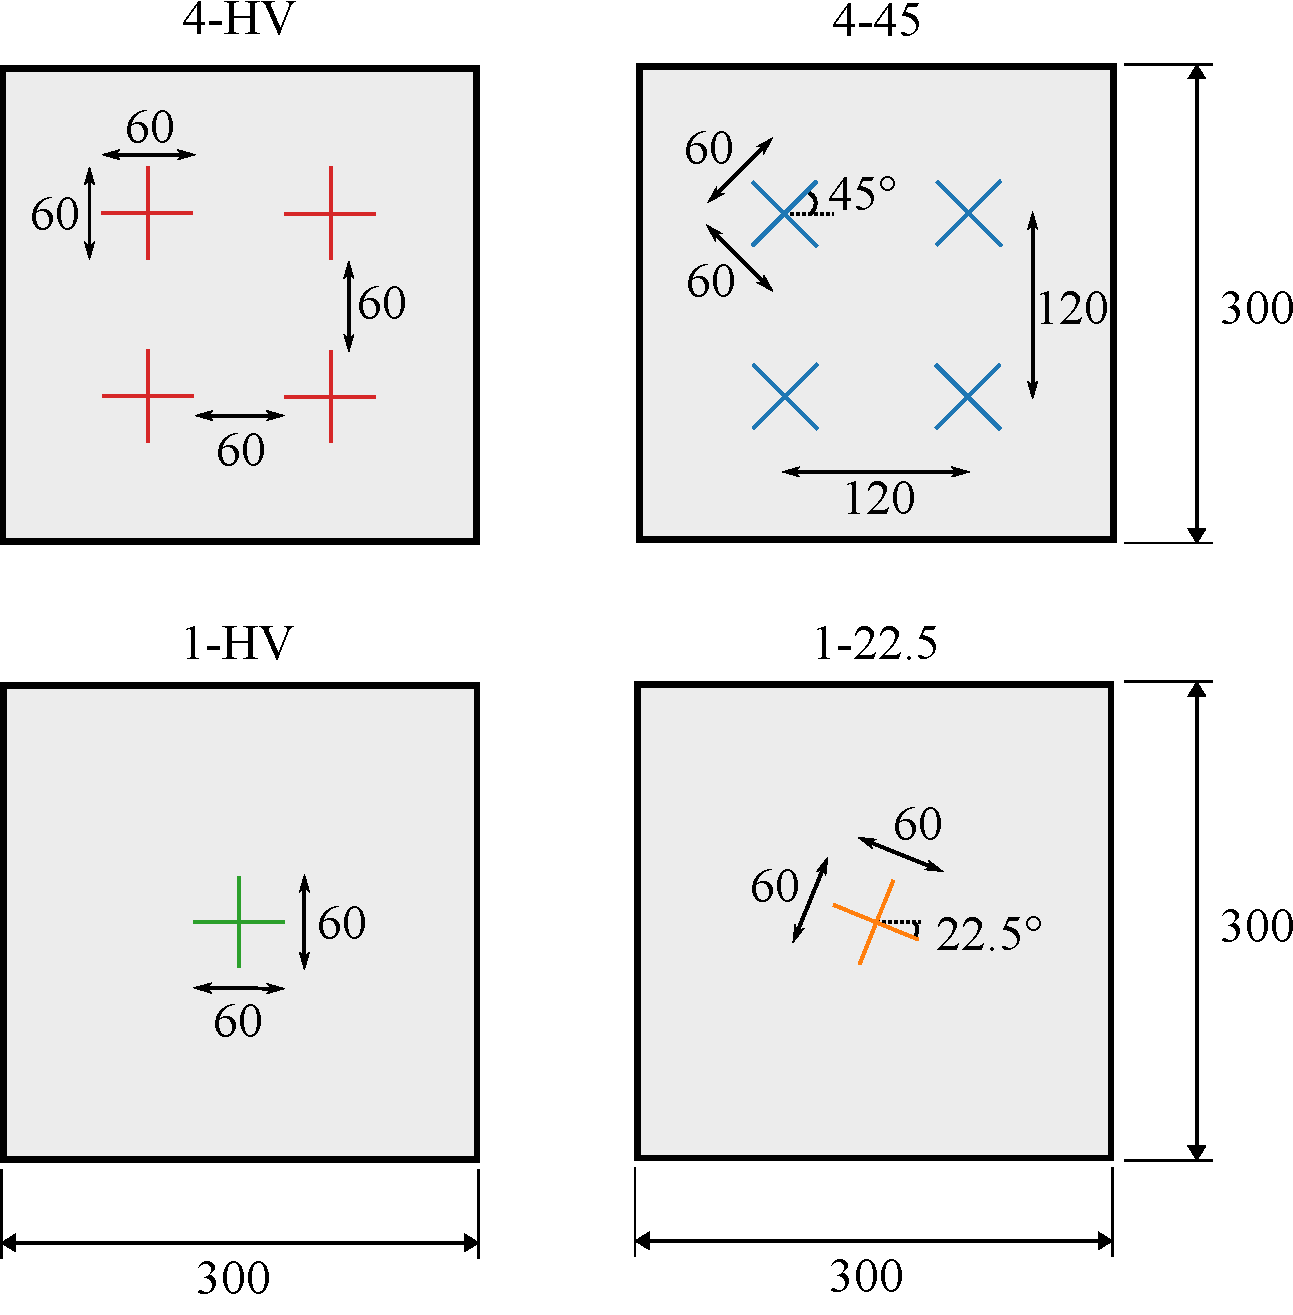
\includegraphics[width=\textwidth]{method/plates}
        \caption{}
        \label{fig:plates}
    \end{subfigure}
    \begin{subfigure}[b]{0.39\textwidth}
        \centering
        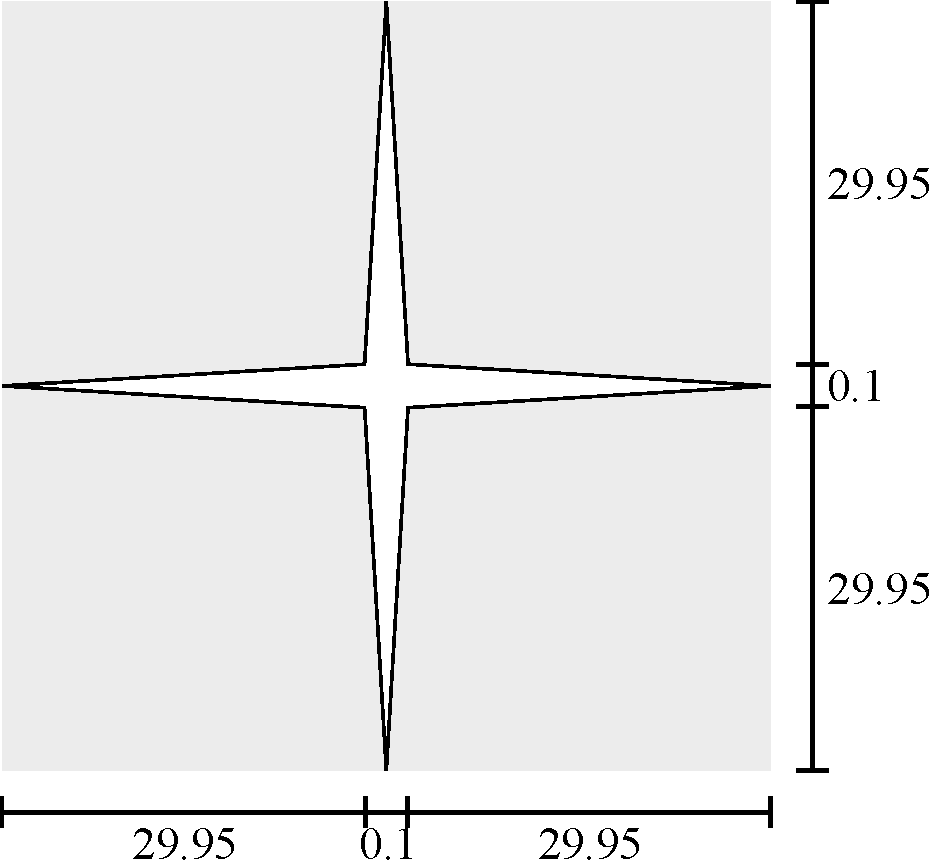
\includegraphics[width=\textwidth]{method/slit}
        \caption{}
        \label{fig:slit}
    \end{subfigure}
    \caption{Sketch of \text{(a)} blast exposed plates with four different slit defect geometries, and \text{(b)} the dimensions of the slits \text{(not drawn to scale)}. Measurements are in mm.}
\end{figure}

\begin{figure}
    \centering
    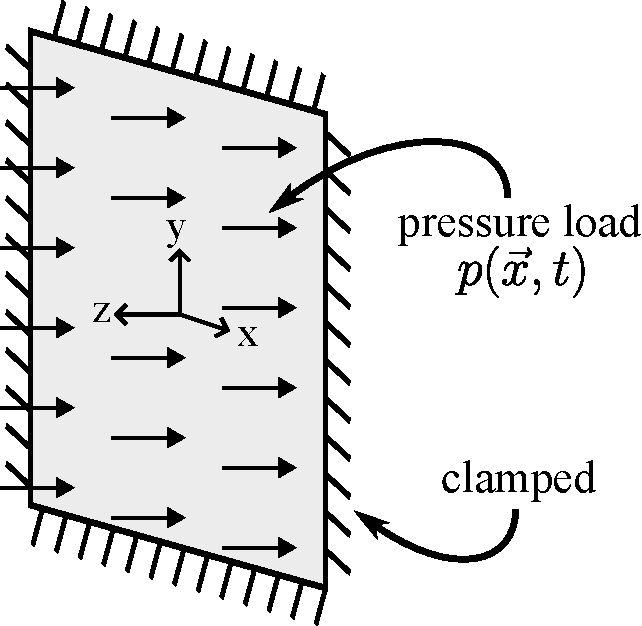
\includegraphics[width=.5\textwidth]{method/BC}
    \caption{Boundary and loading conditions. $p$ denotes pressure applied to one side, $\vec{x}$ denotes the position vector and $t$ is time}
    \label{fig:bc}
\end{figure}

\begin{figure}
    \centering
    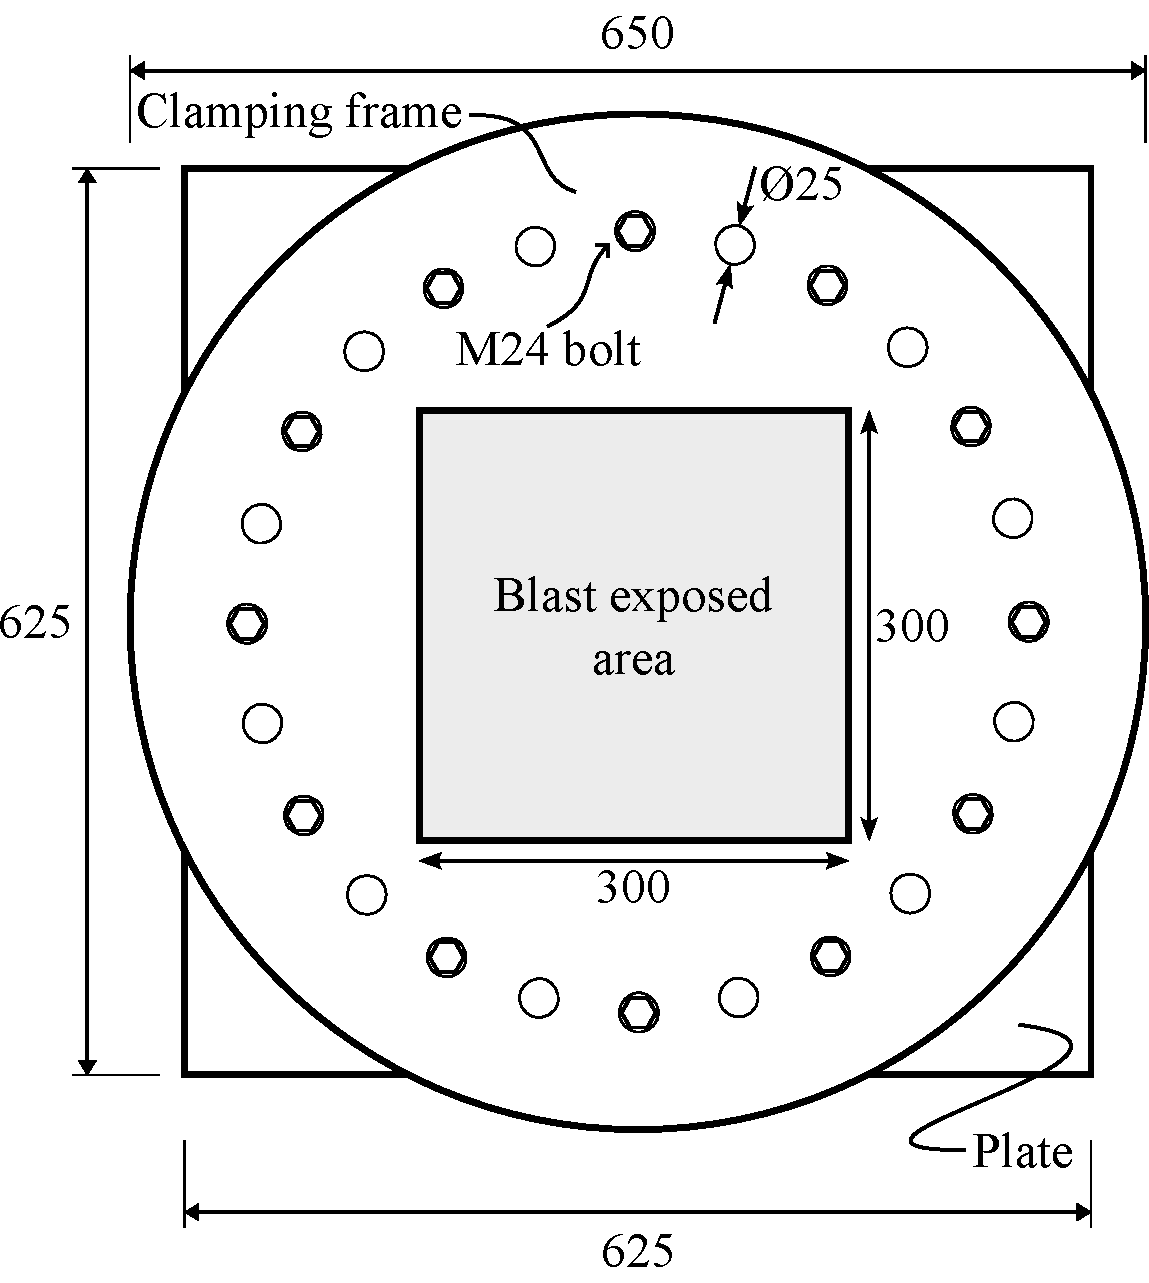
\includegraphics[width=.5\textwidth]{method/clamping_frame}
    \caption{Clamping frame}
    \label{fig:clamping}
\end{figure}
\newpage
\chapter{Results}\label{CH5}
Present the results from following the procedures in \nameref{CH4}, note some observations, but do not discuss them.

\begin{table}[h]
    \centering
    \begin{tabular}{l | l | l}
    A & B & C \\
    \hline
    1 & 2 & 3 \\
    4 & 5 & 6
    \end{tabular}
    \caption{very basic table}
    \label{tab:abc}
    \end{table}

\begin{figure}
    \centering
    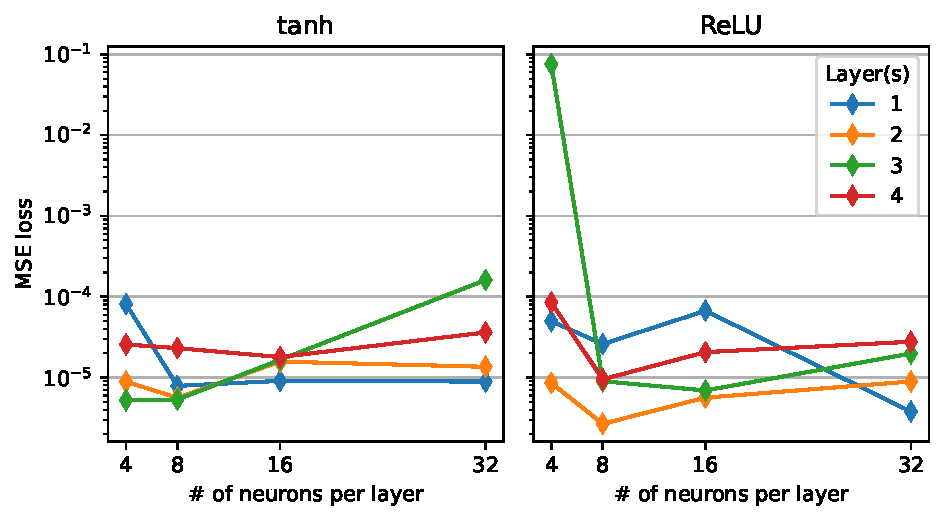
\includegraphics[width=\textwidth]{results/para1_net}
    \caption{Final training losses for different network architectures defined by activation function, number of hidden layers and number of neurons per hidden layer}
    \label{fig:para1_net}
\end{figure}

\begin{figure}
    \centering
    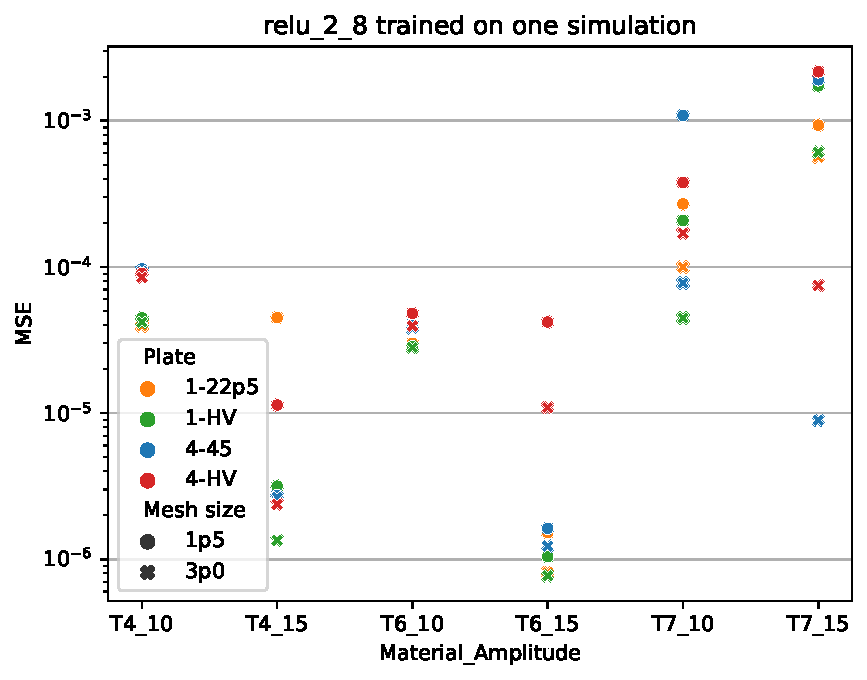
\includegraphics[width=\textwidth]{results/para1_all}
    \caption{Bottom text}
    \label{fig:para1_all}
\end{figure}

\begin{figure}
    \centering
    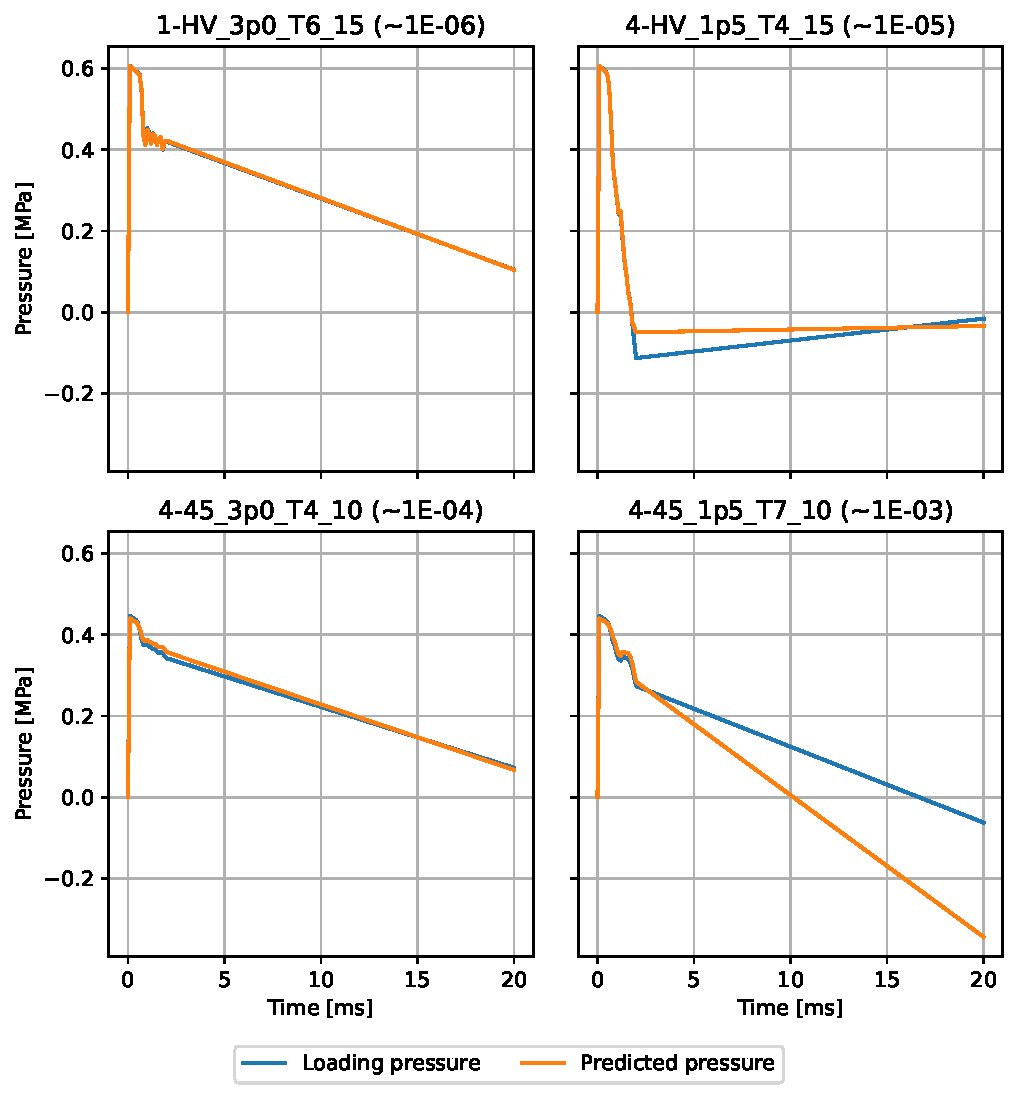
\includegraphics[width=\textwidth]{results/para1_test}
    \caption{Bottom text}
    \label{fig:para1_test}
\end{figure}

\begin{figure}
    \centering
    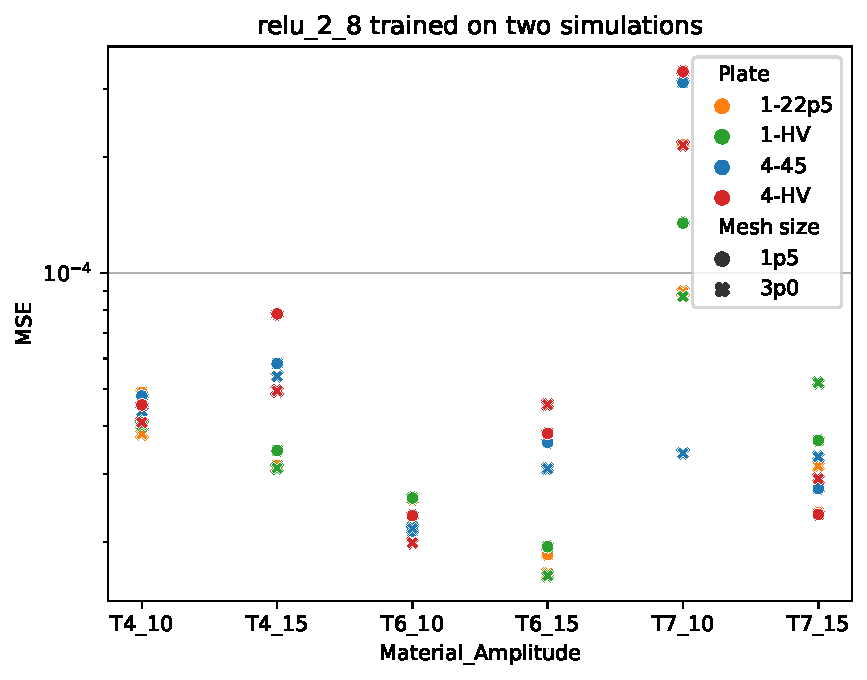
\includegraphics[width=\textwidth]{results/para2_all}
    \caption{Bottom text}
    \label{fig:para2_all}
\end{figure}

\begin{figure}
    \centering
    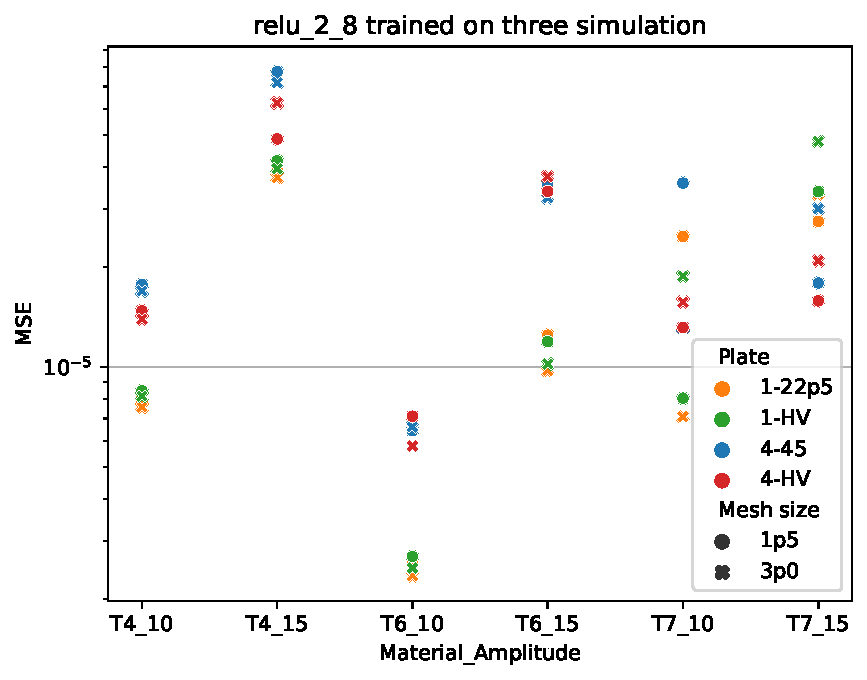
\includegraphics[width=\textwidth]{results/para3_all}
    \caption{Bottom text}
    \label{fig:para3_all}
\end{figure}

\begin{figure}
    \centering
    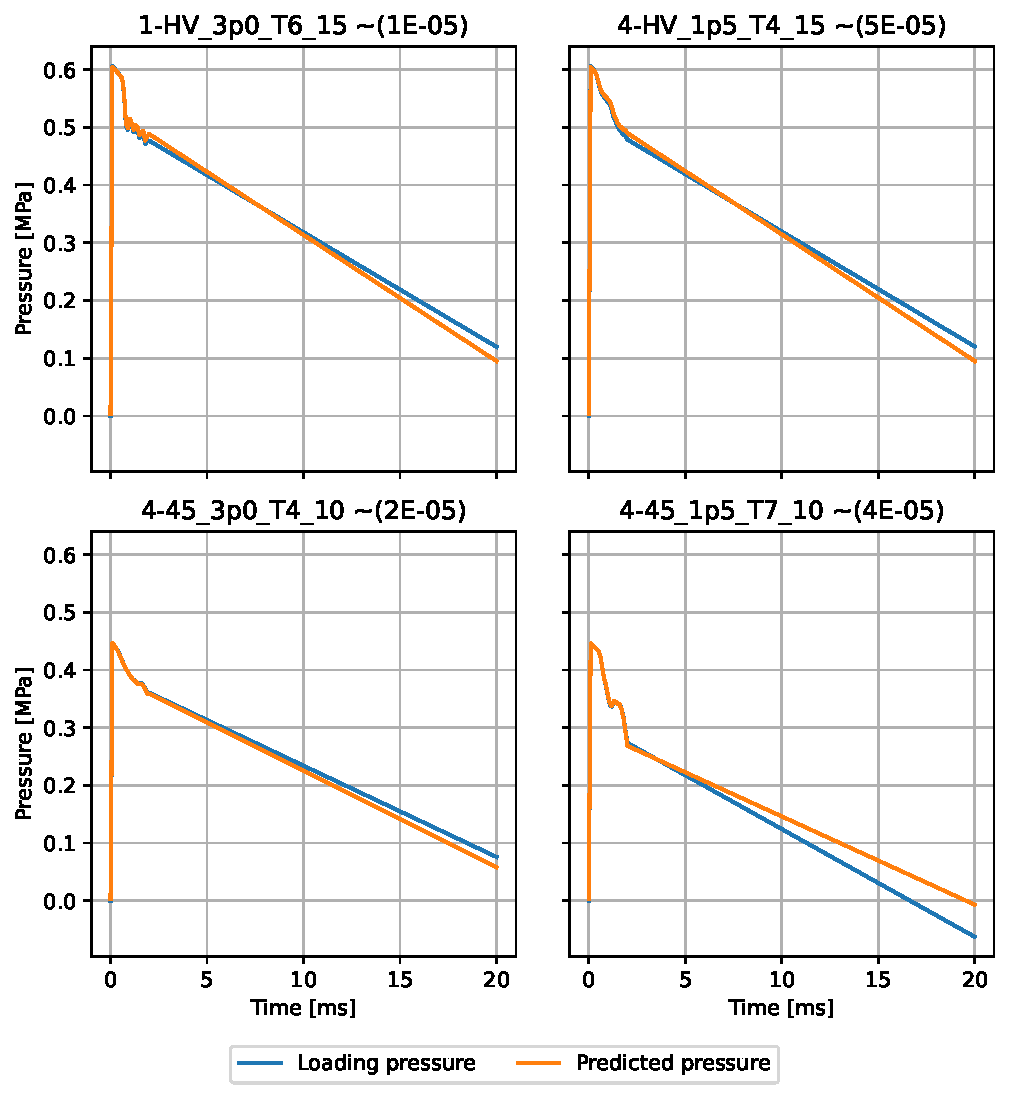
\includegraphics[width=\textwidth]{results/para3_test}
    \caption{Bottom text}
    \label{fig:para3_test}
\end{figure}

\begin{figure}
    \centering
    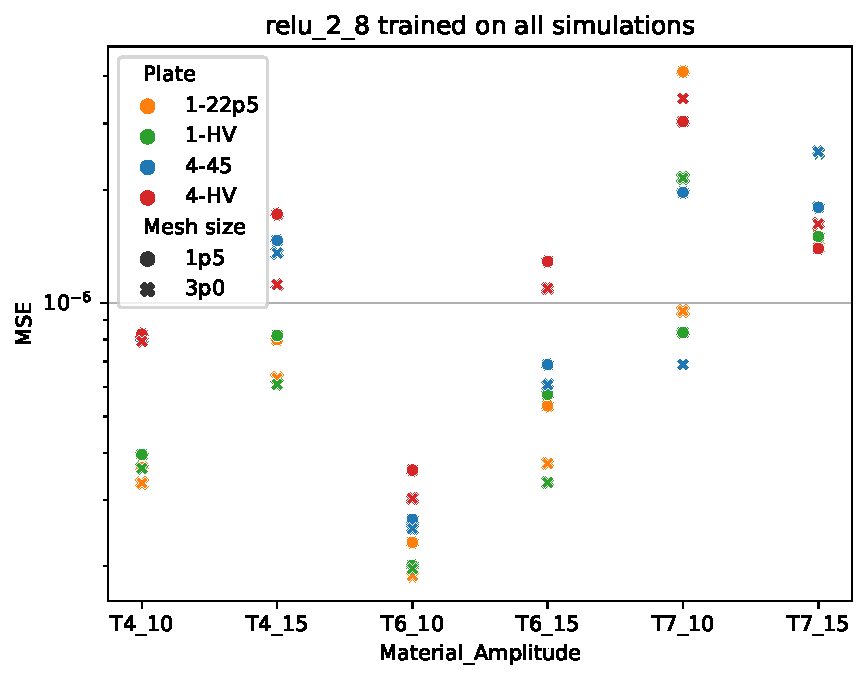
\includegraphics[width=\textwidth]{results/para4_all}
    \caption{Bottom text}
    \label{fig:para4_all}
\end{figure}

\begin{figure}
    \centering
    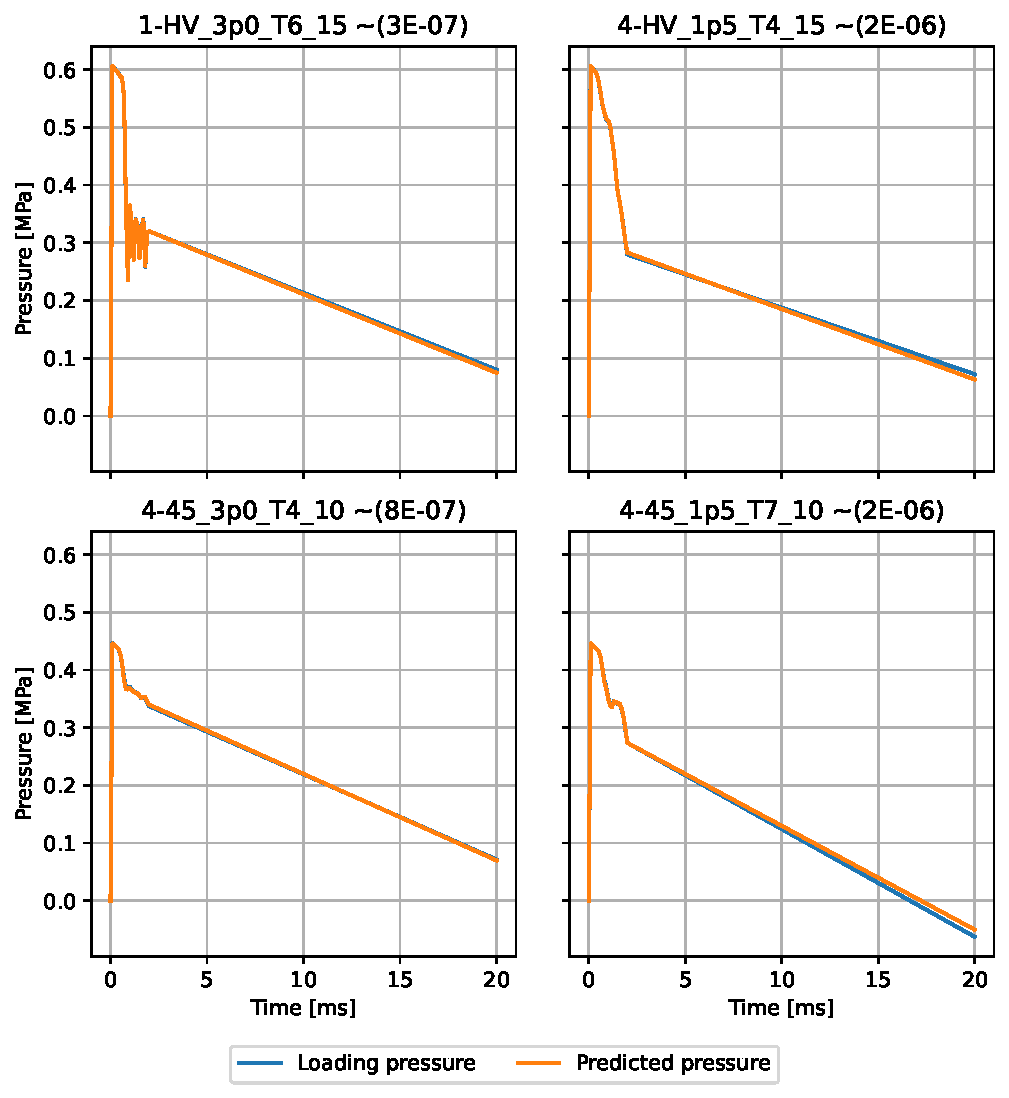
\includegraphics[width=\textwidth]{results/para4_test}
    \caption{Bottom text}
    \label{fig:para4_test}
\end{figure}

\begin{figure}
    \centering
    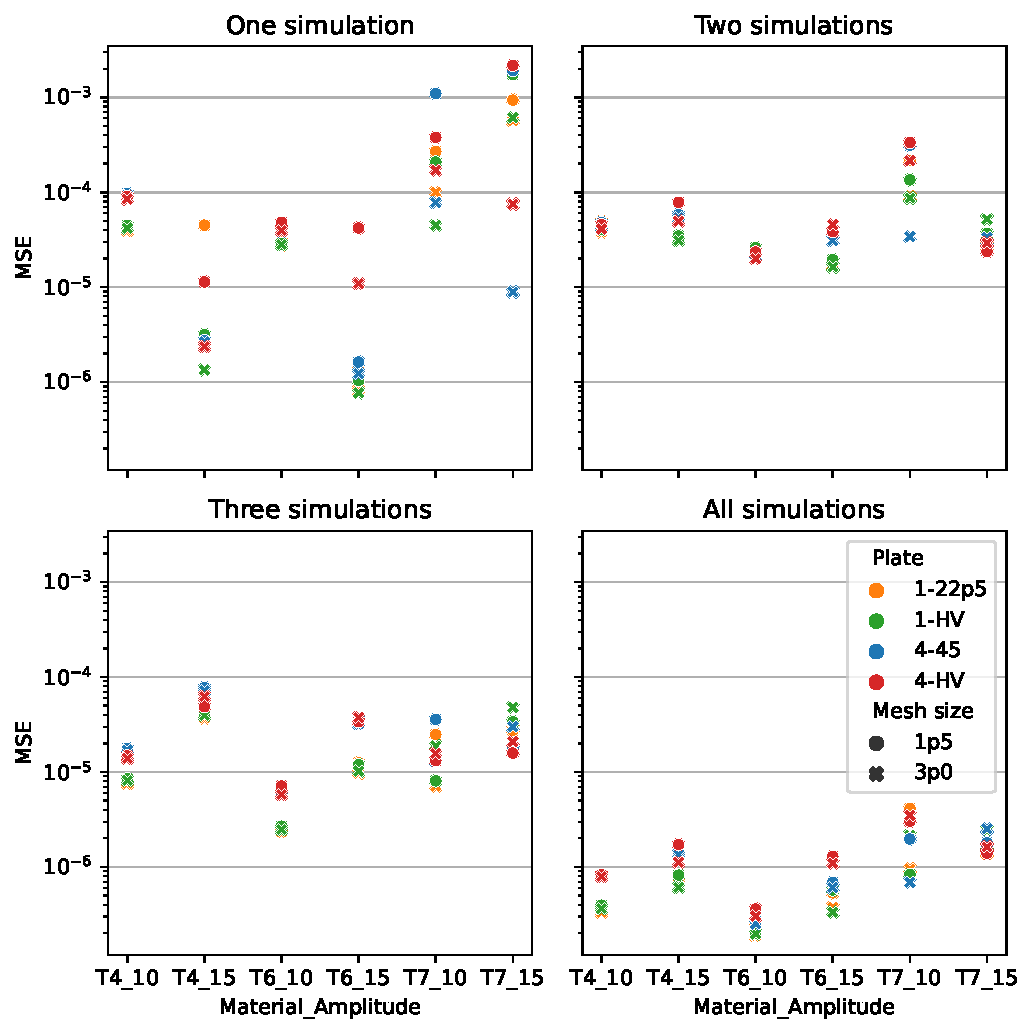
\includegraphics[width=\textwidth]{results/para_all}
    \caption{Bottom text}
    \label{fig:para_all}
\end{figure}

\begin{figure}
    \centering
    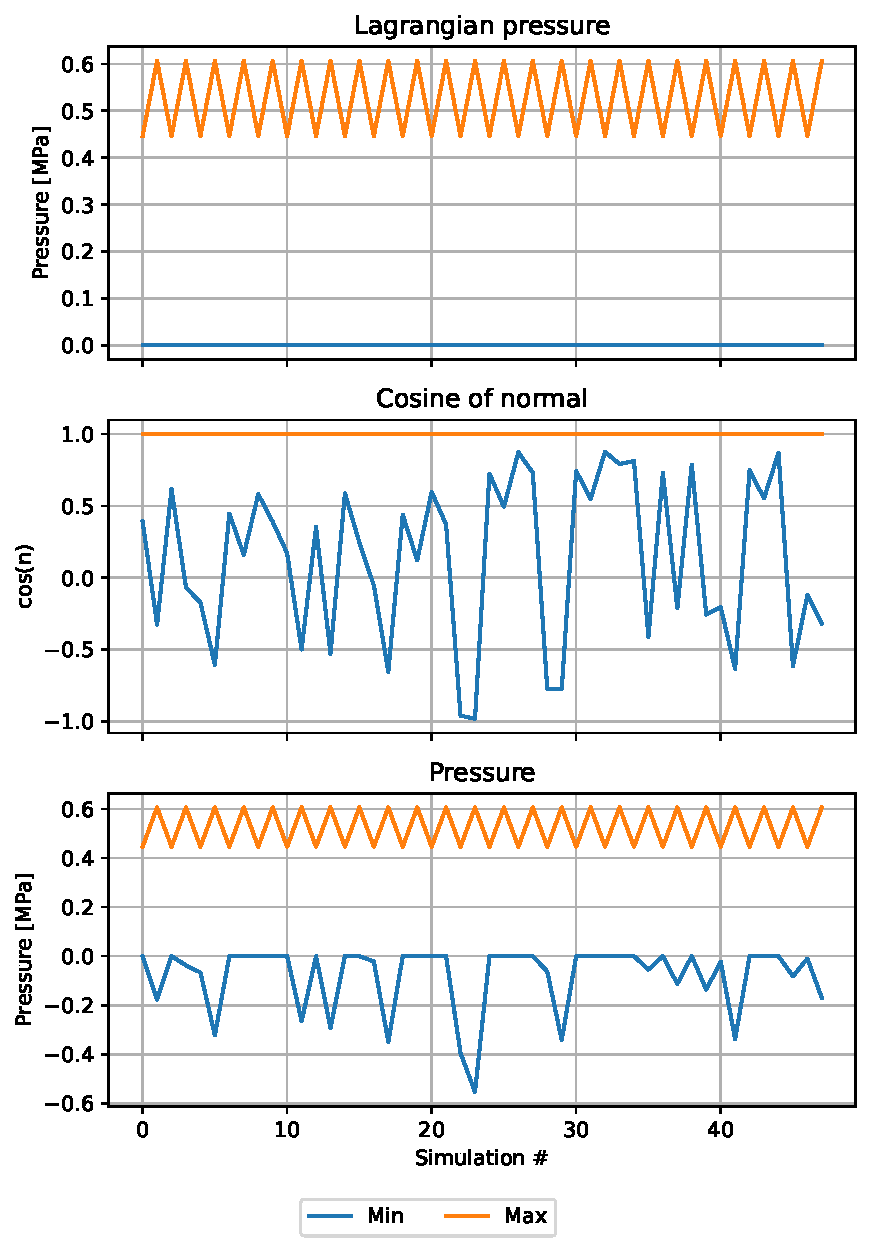
\includegraphics[width=\textwidth]{results/vars}
    \caption{Bottom text}
    \label{fig:para_vars}
\end{figure}

\begin{figure}
    \centering
    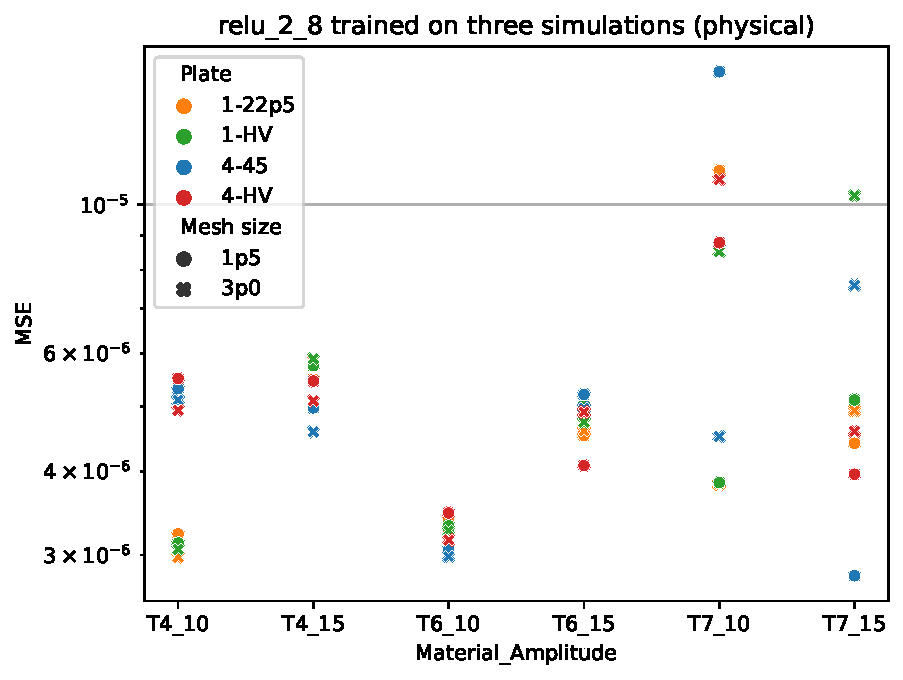
\includegraphics[width=\textwidth]{results/para5_all}
    \caption{Bottom text}
    \label{fig:para5_all}
\end{figure}

\begin{figure}
    \centering
    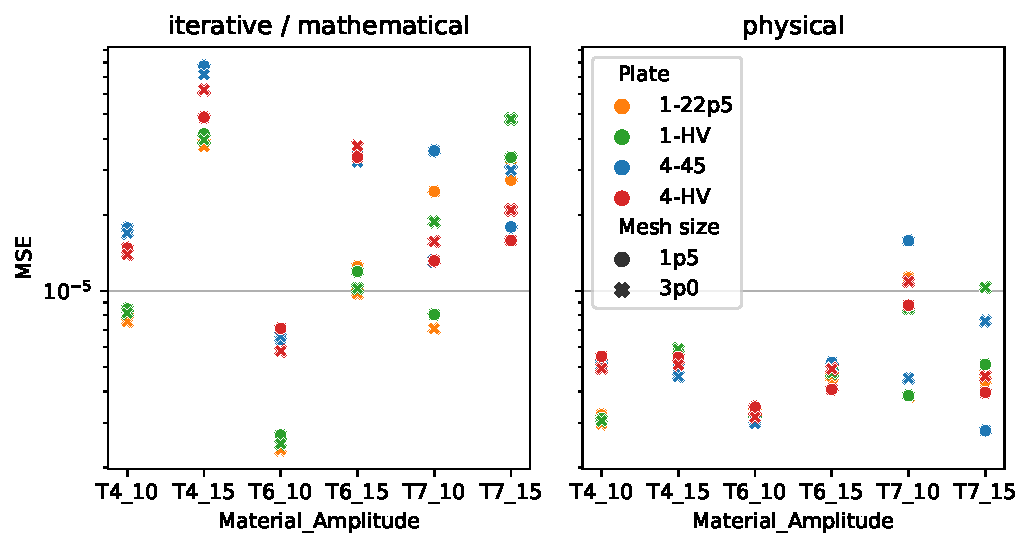
\includegraphics[width=\textwidth]{results/para3_vs_para5}
    \caption{Bottom text}
    \label{fig:para3_vs_para5}
\end{figure}

\begin{figure}
    \centering
    \begin{subfigure}[b]{0.45\textwidth}
        \centering
        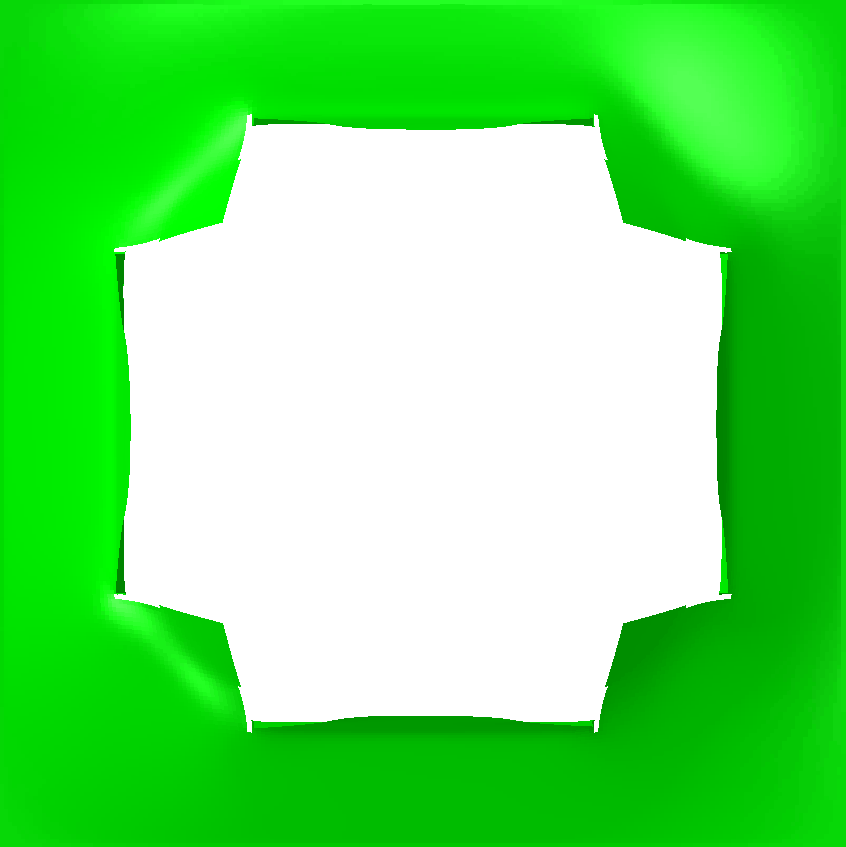
\includegraphics[width=\textwidth]{results/4-HV_1p5_T6_15}
        \caption{test}
        \label{fig:y equals x}
    \end{subfigure}
    \begin{subfigure}[b]{0.45\textwidth}
        \centering
        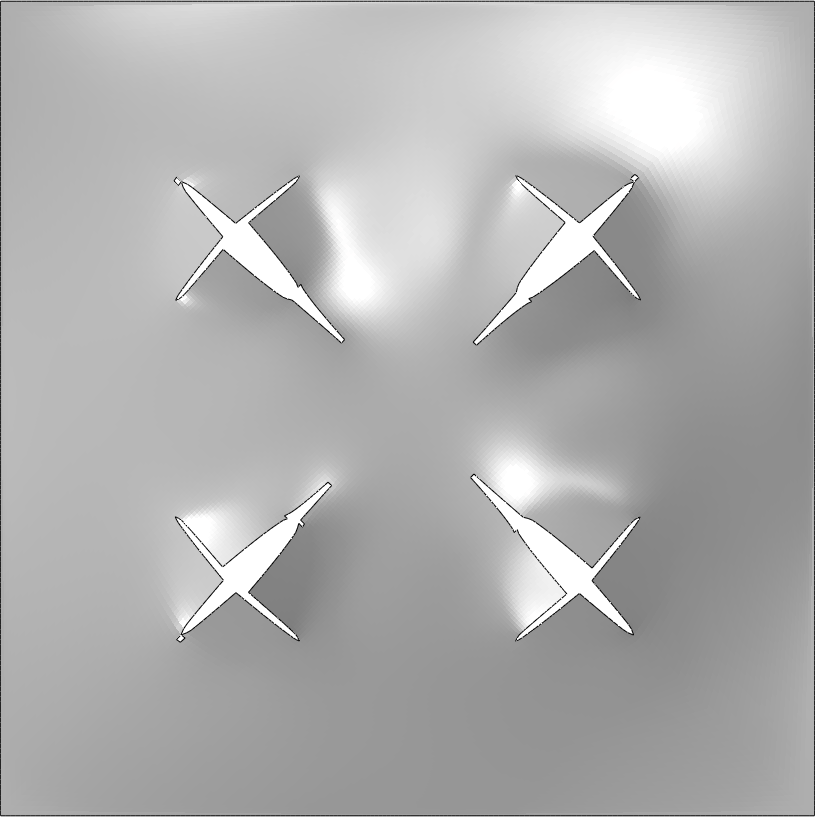
\includegraphics[width=\textwidth]{results/4-45_1p5_T6_15}
        \caption{test}
        \label{fig:three sin x}
    \end{subfigure}
    \begin{subfigure}[b]{0.45\textwidth}
        \centering
        
\includegraphics[width=\textwidth]{results/1-HV_1p5_T6_15}
        \caption{test}
        \label{fig:five over x}
    \end{subfigure}
    \begin{subfigure}[b]{0.45\textwidth}
        \centering
        
\includegraphics[width=\textwidth]{results/1-22p5_1p5_T6_15}
        \caption{test}
        \label{fig:blah}
    \end{subfigure}
       \caption{Effect of slits}
       \label{fig:effect_slit}
\end{figure}
\newpage
\chapter{Discussion}\label{chapter:Discussion}
Discuss the results
\newpage
\chapter{Conclusions}\label{CH7}
Conclusion, further work.
% Bibliography - edit references.bib and use the \cite command in text

\appendix
\chapter{Appendix}\label{chapter:Appendix}
Appendix
\begin{figure}
    \centering
    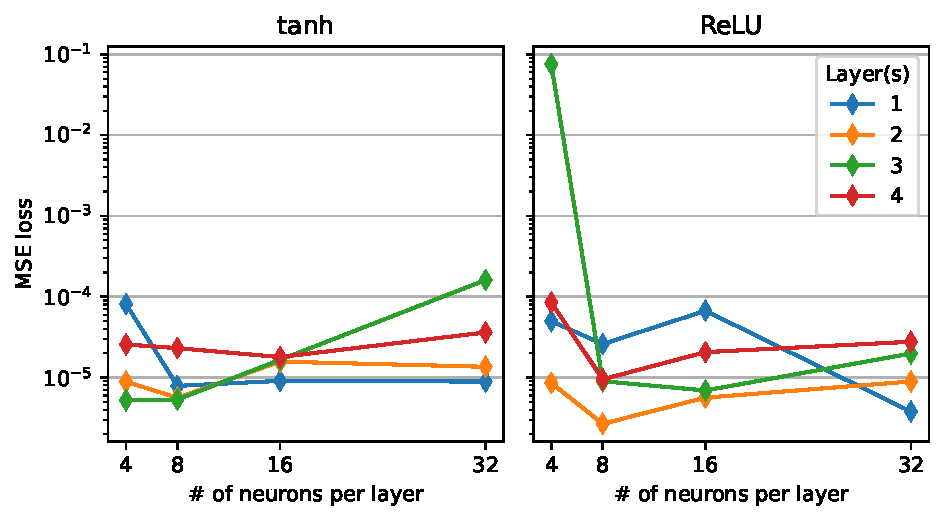
\includegraphics[width=\textwidth]{results/para1_net.pdf}
    \caption{Final training losses for different network architectures defined by activation function, number of hidden layers and number of neurons per hidden layer}
    \label{fig:twqetr}
\end{figure}

\bibliographystyle{unsrt}
\nocite{*}
\bibliography{references}
%Referanselistestil
%\bibliographystyle{IEEEtran}
%\bibliography{IEEEabrv,mybibfile}


\end{document}
